\section{Fixed Controls on Actual Reconstructions}
\label{sec:actualreplay}

A stopping policy must eventually be judged on its reconstructed image,
rather than only on the table used to choose its control. We therefore
replay the sequence-disjoint controls of \cref{sec:crossfit} at the
predeclared QP32 and nominal 0.1\,dB target. Every one of the 53 first frames
is evaluated with mean and Q90 calibration under router, dither and uniform
policies: 318 actual neural reconstructions. The control and exit map are
fixed before the source image is opened for reconstruction and scoring.
No held-out source-error table or quality-based fallback enters this decision.
The checkpoint, sequence folds and development-used corpus remain fixed;
this is not an independent test of trained-router generalisation.

The final reference is the same e15 full-frame reconstruction for every
policy. We report cropped, unclipped equal-channel YCbCr loss and separately
convert and clip RGB before computing its MSE-ratio loss. The RGB source is
obtained from the archived YCbCr420 input; it is not the original camera RGB.
Against this common reference, mean-calibrated router and dither save
25.675\% and 23.802\% synthesis MACs, at mean RGB losses of 0.08679 and
0.08814\,dB. Q90 calibration changes these values to 16.741\%/14.204\%
and 0.05684/0.05636\,dB. The corresponding RGB target-exceedance counts
are 17/16 under mean control and 4/2 under Q90, each out of 53 images
(\cref{fig:actualreplay}). A mean or quantile calibration target is therefore
not a per-image guarantee.

\paragraph{A positive average is not a resolved routing advantage.}
The paired router-minus-dither saving is 1.87 percentage points under mean
control, with a 95\% sequence-bootstrap interval of $[-1.60,5.19]$.
Under Q90 it is 2.54 points, with interval $[-0.42,5.54]$.
Both include zero. Moreover, equal control targets do not enforce equal
achieved RGB quality. We retain all sequences and report these intervals;
this replay does not establish a positive equal-quality routing premium.
It complements, rather than replaces, the per-source retrospective
delivered-cap comparison in the main paper.

On identical padded support and against the archived scalar reference,
the largest absolute discrepancy between actual replay and the stored
table prediction is $3.96\times10^{-4}$\,dB across all 318 cases.
This is a numerical consistency observation. It does not separate backend
differences from mixed-head interactions, nor validate entropy-stream
decodability. The experiment reconstructs neural outputs on CPU; it is
neither a native GPU bitstream test nor a latency measurement.

\paragraph{Recompute the predictor, not only its saved decisions.}
A second CPU audit reloads the frozen codec and router checkpoints and
recomputes source analysis, shared-stem features and router logits on all
53 frames. Historical GPU and current CPU log-probabilities are not exactly
equal: their largest absolute difference is 0.02266. Nevertheless, both
fixed cross-fit controls reproduce every exit decision: zero changed tiles
out of 1,765 under either mean or Q90 control. This validates the replayed
maps at these particular settings, not every control value, QP or backend.
Forward hooks count 289.715 router Conv2d/Linear MACs per padded image pixel.
Pooling, normalisation, nonlinearities, selection, memory movement and
dispatch are excluded; this arithmetic count cannot establish router latency.

\begin{figure*}[t]
\centering
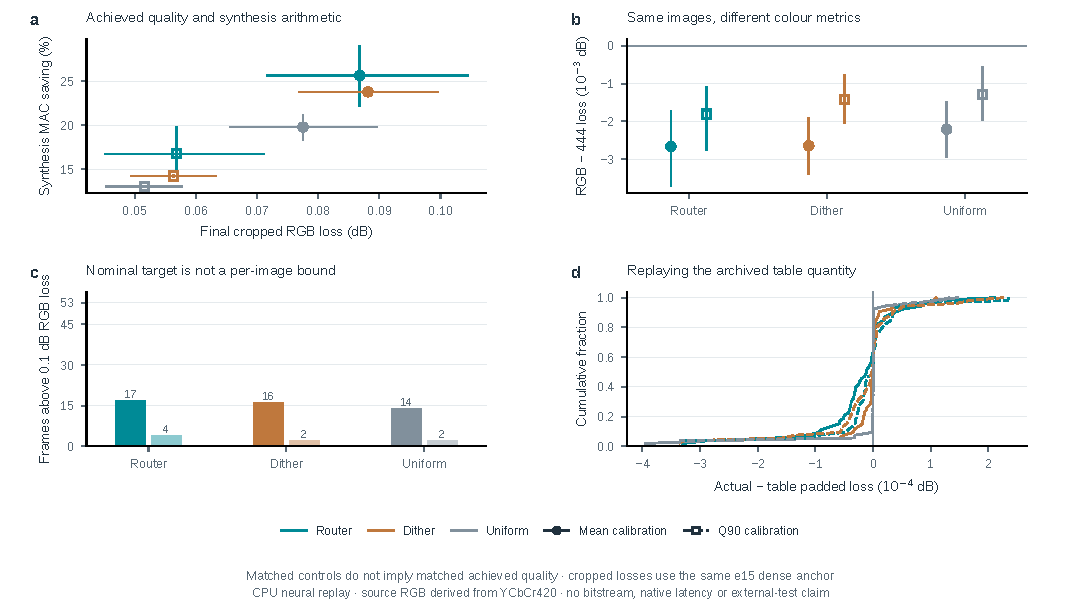
\includegraphics[width=\textwidth]{figs/research20260927/shared_crossfit_qp32/fig_crossfit_actual_replay.pdf}
\caption{\textbf{Carry the fixed decision through to the actual image.}
All 53 sequences at QP32, with no outcome-based exclusions.
\textbf{a}, Achieved RGB loss and synthesis MAC saving with conditional
95\% sequence-bootstrap intervals; these points are not an equal-quality
frontier. \textbf{b}, RGB-minus-444 loss on the same support and reference.
\textbf{c}, Counts above the nominal numerical threshold; pale bars denote
Q90 calibration. \textbf{d}, Actual-minus-table loss on padded support.
Mean and Q90 controls use a different calibration reference and metric from
the cropped RGB report. The paired router--dither saving intervals include
zero under both controls.}
\label{fig:actualreplay}
\end{figure*}

\section{The Cost of Independent Spatial Regions}
\label{sec:patchcontrol}

Shared early exit preserves one encoded representation. A bank of complete
codecs changes that constraint: independently encoded regions can repeat
source context, reset entropy state and introduce additional headers.
Before attributing a gain to expert selection, we measure this cost with
the model held fixed.

We predeclare 16 evenly spaced DIV2K centre crops of size $512\times512$,
five QPs, and three models: D2/D6 at epoch 20 and the released D12 anchor.
Each full-frame reconstruction is compared with four independent
$256\times256$ cores, using source-context halos of 0, 32 or 64 pixels.
These 240 model--image--QP cases retain every variant. A separate decoder
process receives each research bitstream without source pixels; exact
reconstruction, latent, quantised-symbol and entropy-index agreement is
checked. The CPU FP32 FUFREF1 protocol pads images to multiples of 64.
It is not Microsoft's native FP16 CUDA wire format.

\paragraph{Boundary repair can spend more bits than it recovers.}
At 0.2 actual payload bpp, all 16 images are supported by all four D6 curves.
Relative to the same model on the full frame, independent cores lose
0.0611\,dB RGB PSNR; 32- and 64-pixel halos lose 1.2914 and 1.6666\,dB
(\cref{fig:patchrd}). These comparisons interpolate each image in log-rate
space on common measured support, without extrapolation. The respective
95\% paired-image intervals are $[-0.0725,-0.0497]$,
$[-1.4810,-1.1071]$ and $[-1.9113,-1.4178]$\,dB.
They condition on the small fixed cohort and checkpoint, not training seeds.

The same-QP diagnostic explains why a visually improved boundary need not
improve the rate--distortion comparison. At D6/QP32, halo32 changes mean
PSNR by only $+0.0020$\,dB, while increasing payload by 39.72\% on average;
halo64 changes it by $-0.0037$\,dB and increases payload by 57.62\%.
The boundary-specific excess MSE falls towards zero, but the context is
still coded and transmitted (\cref{fig:patchmechanism}). This is a joint
effect of region support, entropy resets and redundant context, not an
isolated causal estimate for one component.

For halo32, each 288-square window is padded to 320; halo64 uses a 320-square
window directly. Both therefore process 1.5625 times the full-frame area,
although their actual source support and coded payload differ. Four FUFREF1
headers occupy 352 bytes versus 88 bytes for the full frame, an additional
0.00806\,bpp at this crop size. At 0.2 complete-container bpp, the D6
core-only loss is 0.2230\,dB on the 15-image common support. The research
identity headers are intentionally explicit and are not a minimum
production signalling format.

\begin{figure*}[t]
\centering
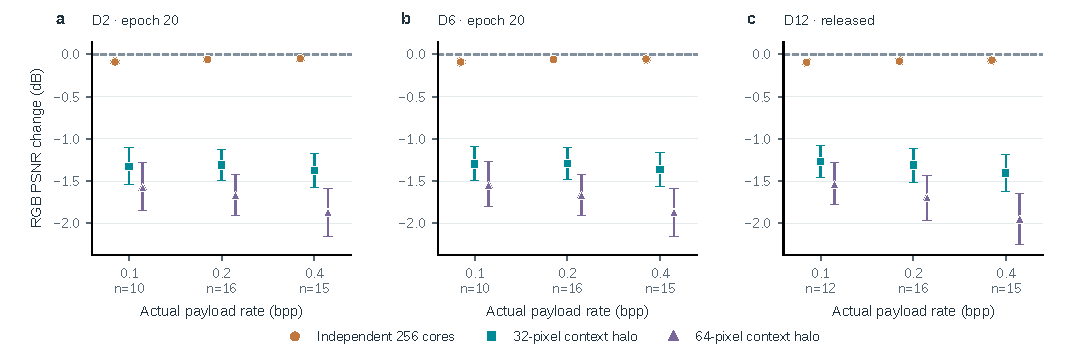
\includegraphics[width=\textwidth]{figs/research20260927/patch_control_epoch020/fig_patch_matched_rate.pdf}
\caption{\textbf{Charge repeated context to the transmitted rate.}
RGB PSNR changes from the same full-frame model at matched actual payload
rate. Each depth uses the common supported images across full frame and all
three patch variants; counts are shown and the vertical scale is shared.
Intervals resample paired images. D2/D6 are interim epoch 20 models; D12 has
different released training provenance. The experiment holds depth fixed
within every contrast and makes no adaptive-routing or runtime claim.}
\label{fig:patchrd}
\end{figure*}

\begin{figure*}[t]
\centering
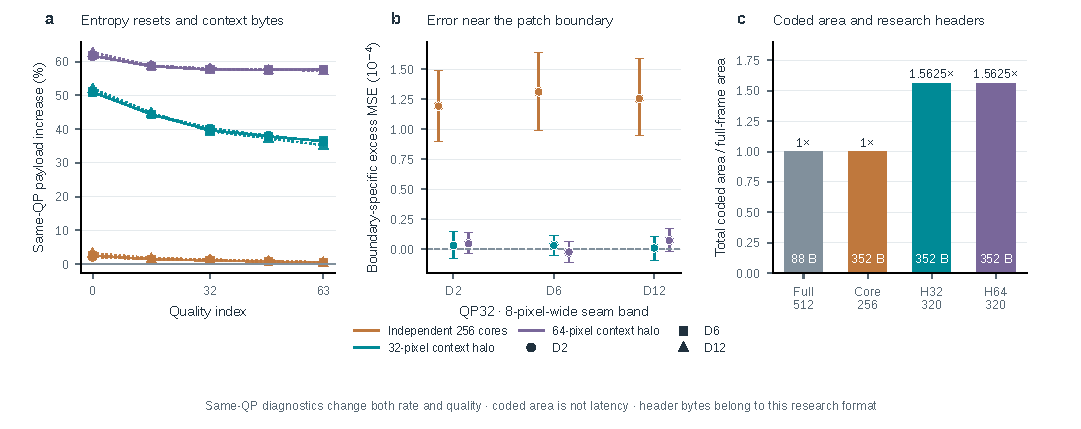
\includegraphics[width=\textwidth]{figs/research20260927/patch_control_epoch020/fig_patch_mechanism.pdf}
\caption{\textbf{A better seam and a better codec are different outcomes.}
\textbf{a}, Same-QP payload increase over the full-frame model.
\textbf{b}, At QP32, patch-minus-full MSE in the central 8-pixel seam band,
minus the corresponding interior excess. \textbf{c}, Exact coded area and
research-header bytes. Halo32 and halo64 have equal coded area under this
padding policy, but different real context. Area ratios are not latency
ratios, and same-QP seam diagnostics are not equal-rate quality comparisons.}
\label{fig:patchmechanism}
\end{figure*}

\begin{figure*}[t]
\centering
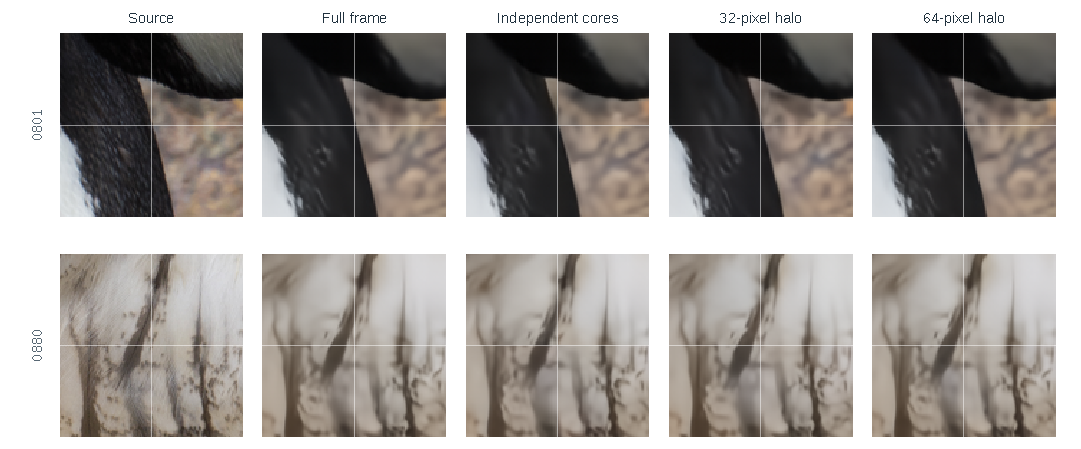
\includegraphics[width=\textwidth]{figs/research20260927/patch_control_epoch020/fig_patch_visual_check.pdf}
\caption{\textbf{Predeclared views at the region intersection.}
D6 epoch 20, QP32, DIV2K 0801 and 0880. All panels use rows and columns 192:320
of the same 512-square crop; images and window were fixed before outcomes.
The common light cross marks the patch boundary. Display images are rounded
to 8 bit; numerical metrics use floating-point RGB. These are same-QP views,
not equal-bitrate reconstructions.}
\label{fig:patchvisual}
\end{figure*}

The practical implication is to evaluate how regions are executed alongside
which expert is assigned. A shallow bank cannot recover its expected cost
advantage merely by adding context everywhere. Padding location and
coalescing of adjacent same-depth regions are separate, predeclared controls;
they must preserve the selected pixel depths and account for all coded bytes.

\subsection{Padding location changes the rate penalty}
The first control rounds a 288-square context window to 320 pixels before
analysis. We repeat all 240 cases with a different geometry: keep the image
at 288 pixels and pad its 18-square latent to 20 before hyperanalysis.
This matches the native path's spatial rounding convention in the CPU
reference implementation. It is not a native CUDA or FP16 equivalence test.
The aligned full-frame, core-only and halo64 cases remain controls; the
full-frame payload and reconstruction are verified unchanged.

At 0.2 payload bpp, all 16 images support all five variants. Changing the
padding location improves halo32 RGB PSNR by 0.2791, 0.2652 and 0.2470\,dB
for D2, D6 and released D12, respectively
(\cref{fig:nativepadding}). For D6, the paired 95\% interval is
$[0.2354,0.2951]$\,dB. This recovery does not remove the cost of independently
coded context: the corrected halo32 path still trails the same full-frame
D6 by 1.0262\,dB, with interval $[0.8614,1.1915]$.
At QP32, the geometry change reduces payload by 6.03\% while changing
mean PSNR by $-0.0055$\,dB. These are distinct comparisons: same-QP byte
reduction and matched-rate quality improvement. Padding location changes
analysis support and hyperprior context together, so the experiment cannot
attribute the effect to either mechanism alone.

\begin{figure*}[t]
\centering
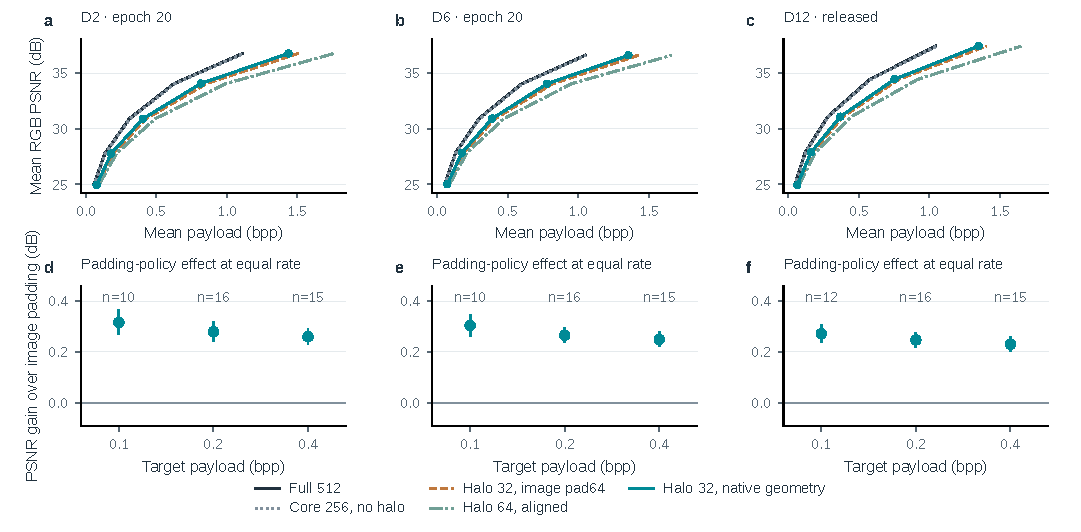
\includegraphics[width=\textwidth]{figs/research20260927/native_padding/fig_native_padding_rd.pdf}
\caption{\textbf{Keep spatial rounding inside the codec contract.}
\textbf{a--c}, Actual-payload RD points averaged over the fixed 16-image
cohort, with shared axis limits. \textbf{d--f}, Per-image matched-rate
gain from moving padding to the latent, with paired 95\% image-bootstrap
intervals. Each rate uses the common support of all five variants within
that depth; $n$ denotes supported images out of 16, with no extrapolation.
The latent-padding implementation uses CPU FP32 research streams;
``native geometry'' does not denote native CUDA output or latency.}
\label{fig:nativepadding}
\end{figure*}

\begin{figure*}[t]
\centering
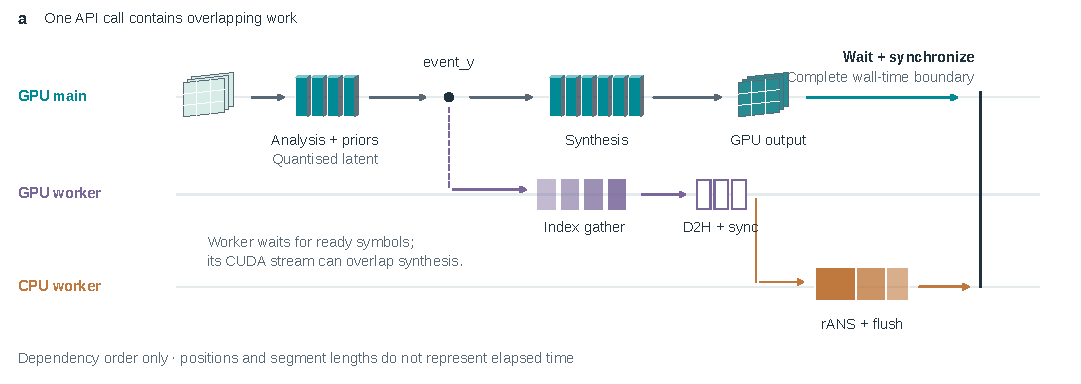
\includegraphics[width=\textwidth]{figs/research20260927/native_execution/fig_native_encoder_dependencies.pdf}
\caption{\textbf{Time the completed workload across streams.}
Source-derived dependencies of the pinned native DCVC-UF intra encoder.
The main-stream reconstruction can overlap worker-stream symbol handling and
CPU entropy coding after the latent-ready event. The right boundary includes
both the worker wait and completion of the GPU reconstruction. Positions,
segment lengths and glyph counts are illustrative, not measured durations
or layer counts. This diagram establishes a timing contract, not a speedup.}
\label{fig:nativeexecution}
\end{figure*}

\subsection{The encoder has a critical path, not a sum of stage costs}
The native intra codec also constrains how an adaptive bank should be timed.
At the pinned Microsoft revision, analysis and prior processing produce the
quantized latent on the main CUDA stream. An event then releases an entropy
worker, while synthesis continues on the main stream. The worker gathers
symbols, transfers them to the host and performs CPU rANS encoding.
The compression call waits for that worker and returns the reconstruction
as a GPU tensor; completing the GPU work requires caller-side synchronization.
Figure~\ref{fig:nativeexecution} records these source-level dependencies.
They permit overlap but do not establish how much overlap occurs on a device.
Consequently, a sum of isolated stage times is not the encoder's elapsed time.

For a resident expert bank, the measurement boundary must additionally include
source-feature extraction, prediction, grouping, expert dispatch and region
assembly. Transfers belong inside that boundary when required by the chosen
output contract. Independently trained experts need their own compatible
latents; choosing a depth does not make their representations interchangeable.
The prepared native correctness harness checks stock versus patched D12 and
fresh-process decoding before any GPU latency claim. Its CPU checkpoint and
CDF preflight has passed; its CUDA execution remains pending.
